After a lot of efforts on optimizing NAMD GPU performance~\cite{phillips_stone_namd_cuda}, NAMD has achieved 
about 10X speed comparing with using one processor-core. However, there is still great
potential space for performance improvement, including tuning on Kepler Tesla K20X and
also improving GPU scalability.

Figures~\ref{figs:apoa1-gpu-singlenode-JYC} and~\ref{figs:apoa1-gpu-scale-JYC}
plot NAMD GPU performance of running the $92K$ atom Apoa1 on a CrayXE/XK machine.
Figure~\ref{figs:apoa1-gpu-singlenode-JYC} shows the performance of running on 
single node with 1 GPU and different numbers of CPU cores. We noticed that increasing
the number of CPU cores actually improves the overall performance up to 5X. Especially, 
using 2 CPU cores provides 2X speedup than using 1 CPU cores.
This is an indication of performance being limited by CPU cores. Furthermore, 
it can be caused by load imbalance between CPU and GPU. In our project, we will profile
and analyze the reason. Hopefully, we will implement a better scheme to balance CPU and GPU load.

Figure~\ref{figs:apoa1-gpu-scale-JYC} illustrates the scalability of 
running Apoa1 simulation on different number of nodes with different configurations of 
(1) GPU with 16 CPU cores(XK7 node), (2) 16 CPU cores only and (3) 32 CPU cores(XE6 node) per node.
On one node, we achieved speed of $3.7x$ and $1.8x$ using GPU, comparing with only using 16 CPU cores
and using 32 CPU cores. However, the benefit of using GPU diminishes with the number of nodes.
Even only on 8 nodes, using GPU does not provide us any improvement compared with using 32 CPU cores.
And the best performance running GPU is only $7.1ms/step$ while it is $2.4$ using 32 CPU cores.
In our project, we will analyze the scaling problem and target at improving GPU scalability.

\begin{figure}[h]
\centering
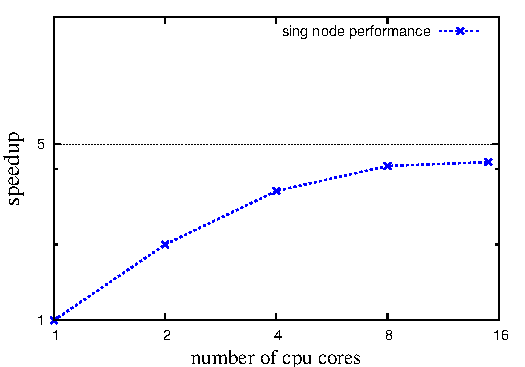
\includegraphics[width=2.8in]{figs/gpu-singlenode}
\caption{Performance of running Apoa1 on one Cray XK7 node using NAMD}
\label{figs:apoa1-gpu-singlenode-JYC}
\vspace{-0.2cm}
\end{figure}

\begin{figure}[h]
\centering
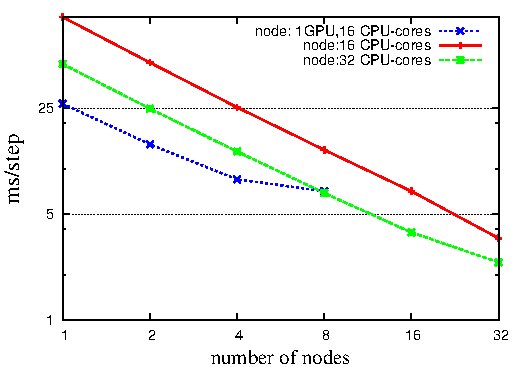
\includegraphics[width=2.8in]{figs/cpu-gpu-jyc-apoa1}
\caption{Scalable performance of running Apoa1 on Cray XK7 and XE6 nodes }
\label{figs:apoa1-gpu-scale-JYC}
\vspace{-0.2cm}
\end{figure}



